\documentclass[tikz,border=0pt]{standalone}
\usepackage[american]{circuitikz}
\usetikzlibrary{arrows.meta,calc,positioning,decorations.pathmorphing,patterns}
\definecolor{zyloTeal}{HTML}{174A5B}
\definecolor{zyloTealTwo}{HTML}{246B7A}
\definecolor{zyloInk}{HTML}{1F2933}
\definecolor{zyloSoft}{HTML}{EAF4F4}
\definecolor{zyloPaper}{HTML}{F8FAFB}
\definecolor{zyloLine}{HTML}{44606B}
\definecolor{zyloOrange}{HTML}{D97706}
\begin{document}
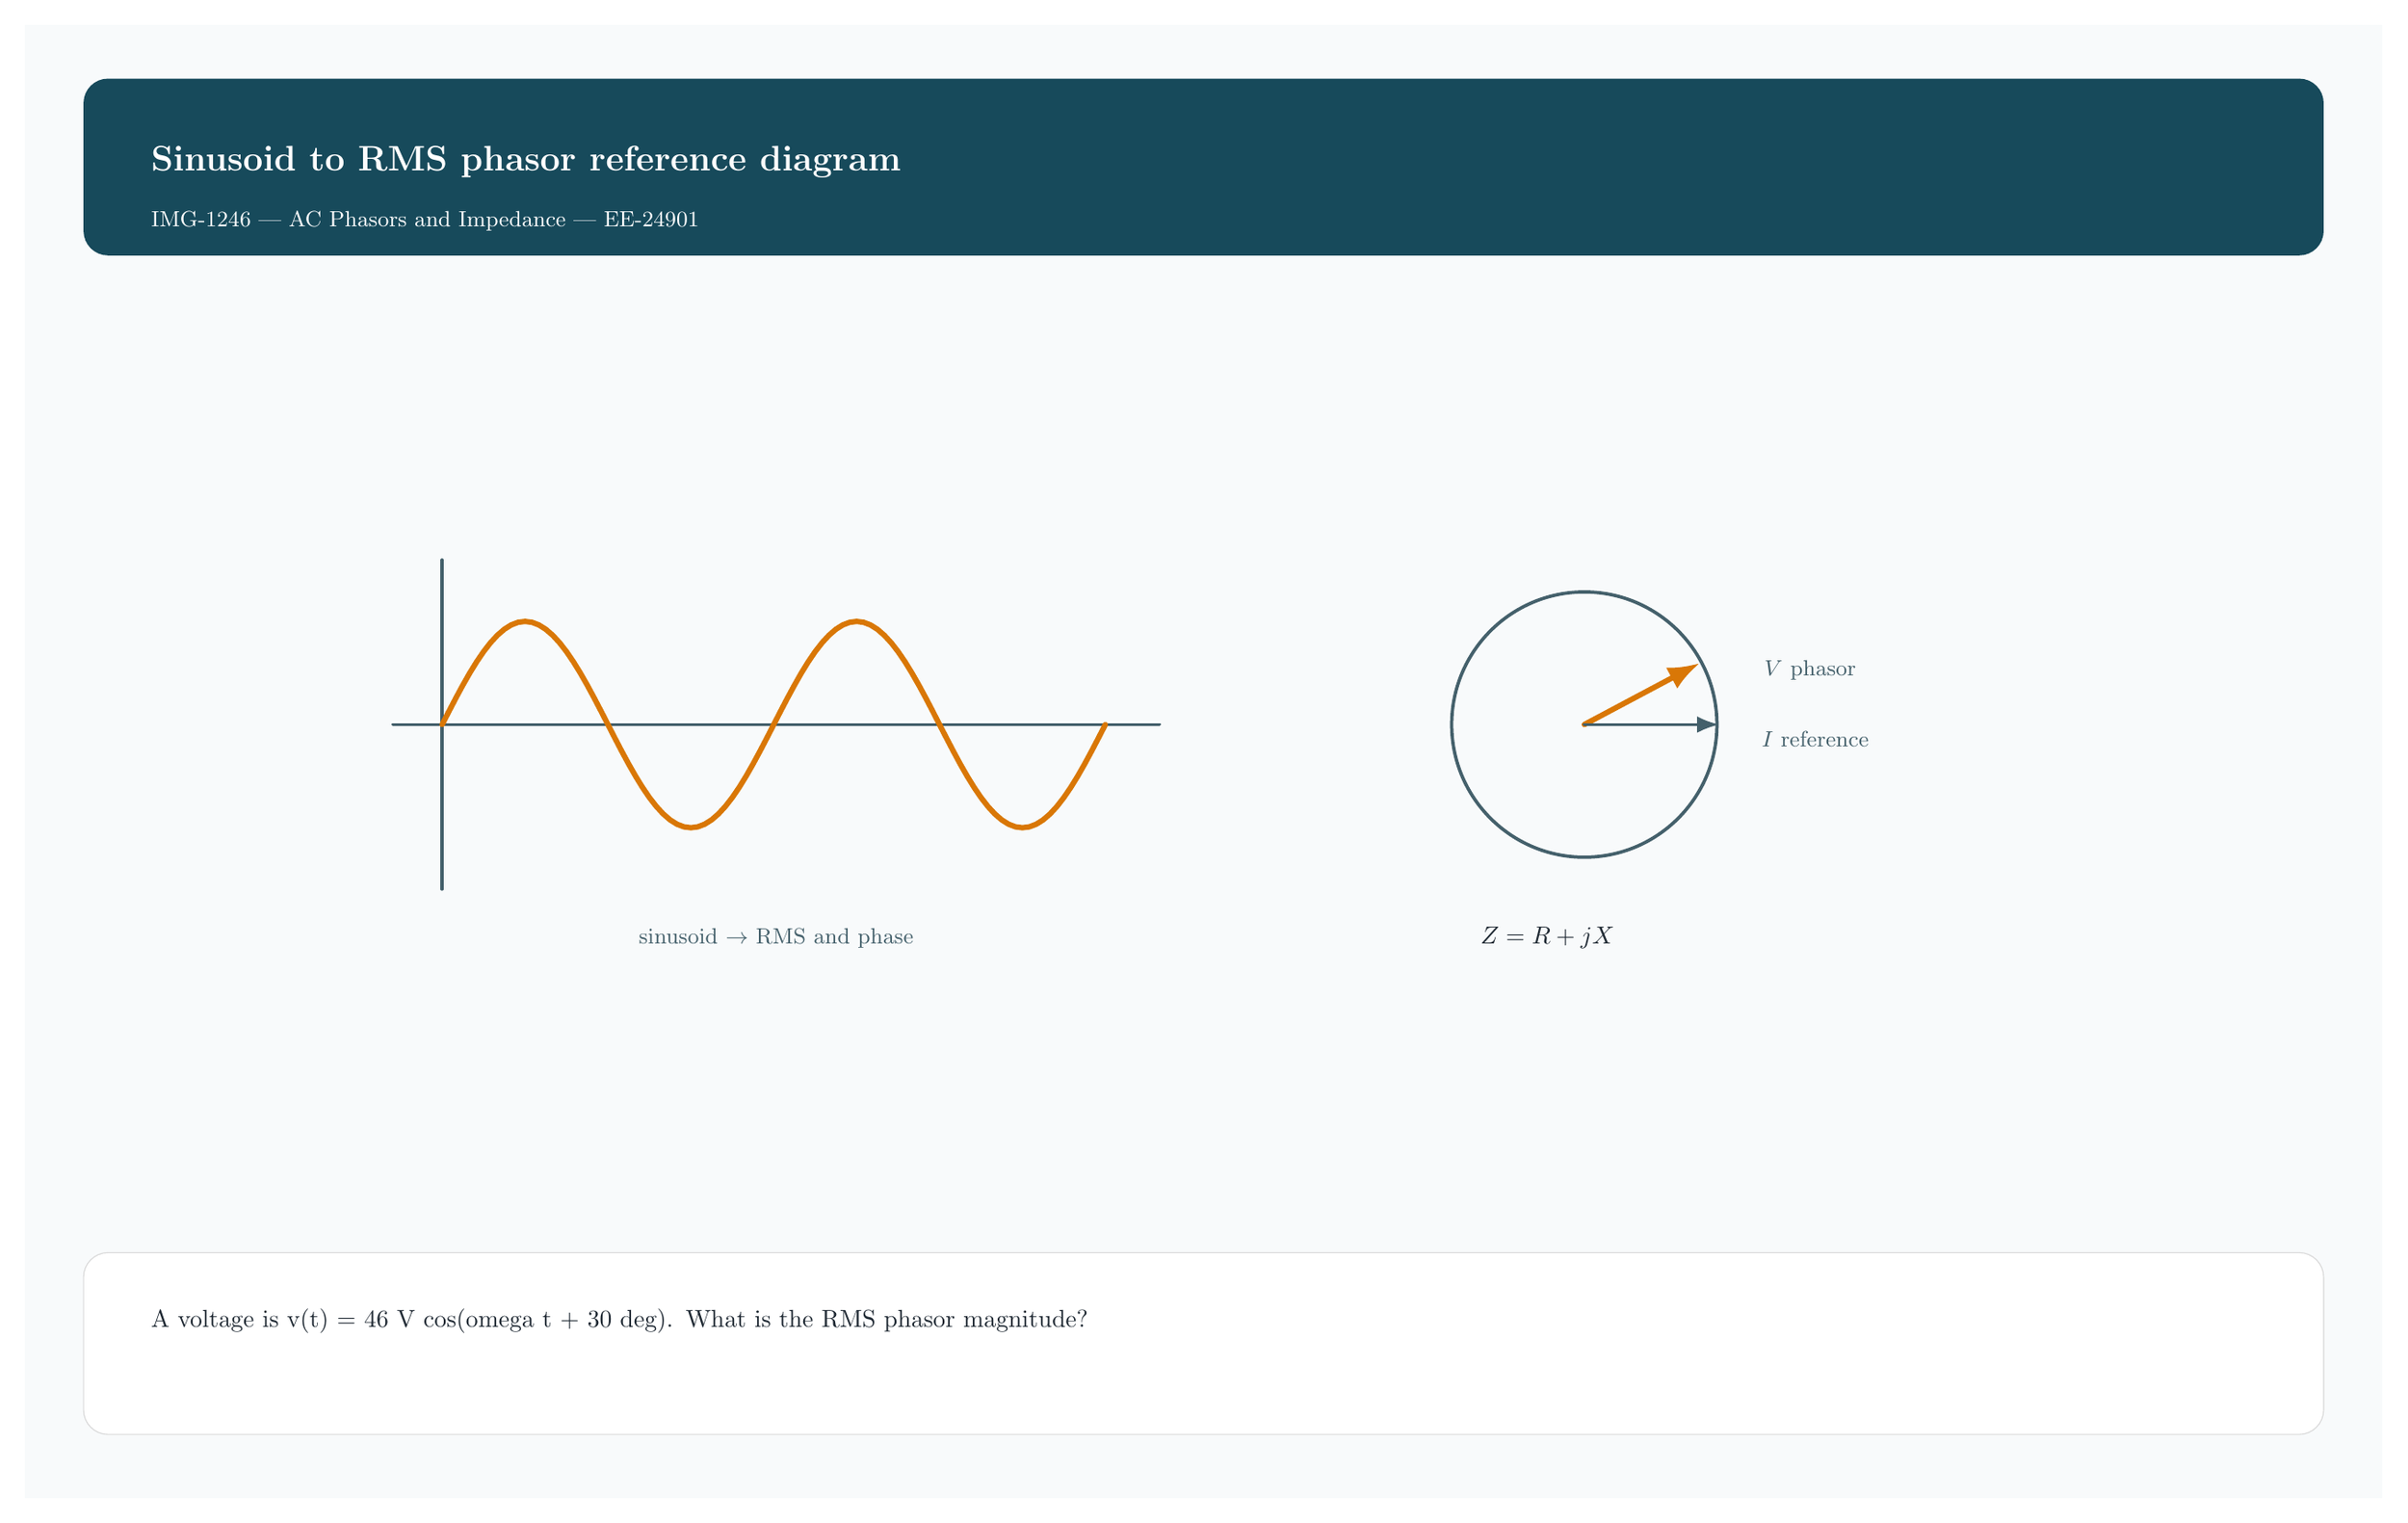
\begin{tikzpicture}[x=1pt,y=-1pt,>=Latex,line cap=round,line join=round]
\path[fill=zyloPaper] (0,0) rectangle (960,600);
\path[fill=zyloTeal,rounded corners=10pt] (24,22) rectangle (936,94);
\node[anchor=west,text=white,font=\bfseries\Large] at (48,56) {Sinusoid to RMS phasor reference diagram};
\node[anchor=west,text=white!82,font=\small] at (48,80) {IMG-1246 | AC Phasors and Impedance | EE-24901};
\tikzset{wire/.style={draw=zyloTeal,line width=2.2pt},thinwire/.style={draw=zyloLine,line width=1.35pt},accent/.style={draw=zyloOrange,line width=2.2pt},box/.style={draw=zyloTealTwo,fill=zyloSoft,line width=1.5pt,rounded corners=8pt}}
\draw[thinwire] (150,285) -- (462,285);
\draw[thinwire] (170,218) -- (170,352);
\draw[accent] (170,285) -- (172.812,279.518) -- (175.625,274.13) -- (178.438,268.927) -- (181.25,264) -- (184.062,259.432) -- (186.875,255.302) -- (189.688,251.679) -- (192.5,248.627) -- (195.312,246.197) -- (198.125,244.431) -- (200.938,243.359) -- (203.75,243) -- (206.562,243.359) -- (209.375,244.431) -- (212.188,246.197) -- (215,248.627) -- (217.812,251.679) -- (220.625,255.302) -- (223.438,259.432) -- (226.25,264) -- (229.062,268.927) -- (231.875,274.13) -- (234.688,279.518) -- (237.5,285) -- (240.312,290.482) -- (243.125,295.87) -- (245.938,301.073) -- (248.75,306) -- (251.562,310.568) -- (254.375,314.698) -- (257.188,318.321) -- (260,321.373) -- (262.812,323.803) -- (265.625,325.569) -- (268.438,326.641) -- (271.25,327) -- (274.062,326.641) -- (276.875,325.569) -- (279.688,323.803) -- (282.5,321.373) -- (285.312,318.321) -- (288.125,314.698) -- (290.938,310.568) -- (293.75,306) -- (296.562,301.073) -- (299.375,295.87) -- (302.188,290.482) -- (305,285) -- (307.812,279.518) -- (310.625,274.13) -- (313.438,268.927) -- (316.25,264) -- (319.062,259.432) -- (321.875,255.302) -- (324.688,251.679) -- (327.5,248.627) -- (330.312,246.197) -- (333.125,244.431) -- (335.938,243.359) -- (338.75,243) -- (341.562,243.359) -- (344.375,244.431) -- (347.188,246.197) -- (350,248.627) -- (352.812,251.679) -- (355.625,255.302) -- (358.438,259.432) -- (361.25,264) -- (364.062,268.927) -- (366.875,274.13) -- (369.688,279.518) -- (372.5,285) -- (375.312,290.482) -- (378.125,295.87) -- (380.938,301.073) -- (383.75,306) -- (386.562,310.568) -- (389.375,314.698) -- (392.188,318.321) -- (395,321.373) -- (397.812,323.803) -- (400.625,325.569) -- (403.438,326.641) -- (406.25,327) -- (409.062,326.641) -- (411.875,325.569) -- (414.688,323.803) -- (417.5,321.373) -- (420.312,318.321) -- (423.125,314.698) -- (425.938,310.568) -- (428.75,306) -- (431.562,301.073) -- (434.375,295.87) -- (437.188,290.482) -- (440,285);
\draw[thinwire] (635,285) circle (54); \draw[accent,->] (635,285) -- (682,260); \draw[thinwire,->] (635,285) -- (690,285);
\node[font=\small,text=zyloLine] at (727,263) {$V$ phasor}; \node[font=\small,text=zyloLine] at (729,291) {$I$ reference};
\node[font=\small,text=zyloLine] at (306,372) {sinusoid $\rightarrow$ RMS and phase}; \node[text=zyloInk] at (620,372) {$Z=R+jX$};
\path[draw=black!15,fill=white,rounded corners=10pt] (24,500) rectangle (936,574);
\node[anchor=west,text width=860pt,align=left,text=zyloInk,font=\normalsize] at (48,528) {A voltage is v(t) = 46 V cos(omega t + 30 deg). What is the RMS phasor magnitude?};
\end{tikzpicture}
\end{document}
